\documentclass{article}


\usepackage{subcaption}
\usepackage{circuitikz}
\usepackage[T1]{fontenc} 
\usepackage[utf8]{inputenc}
\usepackage{amsmath}
\usepackage{amssymb}
\usepackage{fancyhdr}
\usepackage{graphicx}
\usepackage{hyperref}
\usepackage{tikz}
  \usetikzlibrary{arrows}
  \usetikzlibrary{shapes}
  \usetikzlibrary{arrows.meta,topaths}
  \usetikzlibrary{bending}
  \usetikzlibrary{calc}
\usepackage{anyfontsize}
\usepackage{sectsty}
\usepackage{../assets/scripts/tex/color-env}
\usepackage{anyfontsize}
\usepackage{xcolor}
\definecolor{DarkGreenBlue}{HTML}{264653}
\definecolor{LightGreenBlue}{HTML}{2A9D8F}
\definecolor{LightOrange}{HTML}{E9C46A}
\definecolor{DarkOrange}{HTML}{F4A261}
\definecolor{RedOrange}{HTML}{E76F51}
\definecolor{BrightRed}{HTML}{D62828}
\definecolor{DeepBlue}{HTML}{003049}



\usepackage[ngerman]{babel}
\title{Elektrotechnik 1 - Praktikum 3}


\usepackage[
  includehead,
  headheight = 17mm,
  footskip = \dimexpr\headsep+\ht\strutbox\relax,
  tmargin = 0mm,
  bmargin = \dimexpr17mm+2\ht\strutbox\relax,
]{geometry}





\pagestyle{fancy}
\fancyhead[L]{\leftmark}
\fancyhead[R]{}
\fancyfoot[L]{}
\fancyfoot[C]{\thepage}
\fancyfoot[R]{
\includegraphics[scale=0.2]{../assets/images/haw.jpg}}
\renewcommand\headrulewidth{0.5pt}

\begin{document}

\thispagestyle{empty}
\begin{tikzpicture}[remember picture,overlay]

  \fill[DeepBlue] (current page.south west) rectangle (current page.north east);

  \begin{scope}

    \foreach \i in {2.5,...,22}
      {
        \node[rounded corners, DeepBlue!90,draw ,regular polygon, regular polygon sides=6, minimum size=\i cm, ultra thick] at ($(current page.west)+(2.5,-5)$) {} ;
      }

  \end{scope}

  \node[rounded corners,fill=DeepBlue!95,text =DeepBlue!5,regular polygon,regular polygon sides=6, minimum size=2.5 cm,inner sep=0,ultra thick] at ($(current page.west)+(2.5,-5)$) {\LARGE \bfseries 2020};

  \foreach \i in {0.5,...,22}
    {
      \node[rounded corners,DeepBlue!90,draw,regular polygon,regular polygon sides=6, minimum size=\i cm,ultra thick] at ($(current page.north west)+(2.5,0)$) {} ;
    }

  \foreach \i in {0.5,...,22}
    {
      \node[rounded corners,DeepBlue!98,draw,regular polygon,regular polygon sides=6, minimum size=\i cm,ultra thick] at ($(current page.north east)+(0,-9.5)$) {} ;
    }

  \foreach \i in {12}
    {
      \node[fill = DeepBlue,rounded corners,draw=DeepBlue,regular polygon,regular polygon sides=6, minimum size=\i cm,ultra thick] at ($(current page.south east)+(-0.2,-0.45)$) {} ;
    }


  \foreach \i in {21,...,6}
    {
      \node[DeepBlue!95,rounded corners,draw,regular polygon,regular polygon sides=6, minimum size=\i cm,ultra thick] at ($(current page.south east)+(-0.2,-0.45)$) {} ;
    }

  \node[left,DeepBlue!5,minimum width=0.625*\paperwidth,minimum height=3cm, rounded corners] at ($(current page.north east)+(0,-9.5)$){{\fontsize{25}{30} \selectfont \bfseries ET2 - Praktikum 7}};

  \node[left,DeepBlue!10,minimum width=0.625*\paperwidth,minimum height=2cm, rounded corners] at ($(current page.north east)+(0,-11)$){{\huge \textit{Matlab}}};

  \node[left,DeepBlue!5,minimum width=0.625*\paperwidth,minimum height=2cm, rounded corners] at ($(current page.north east)+(0,-13)$){{\Large \textsc{Florian Tietjen\hspace{0.5cm}Eric Antosch}}};

\end{tikzpicture}

\newpage
\thispagestyle{empty}

\tableofcontents


\newpage

\section{Aufgabe 1: Variablen}

\begin{task}
  TIn der ersten Aufgabe geht es um das Anlegen von Variablen und das Arbeiten mit eben jenen Werten.
\end{task}


\begin{figure}[h]
  \centering
  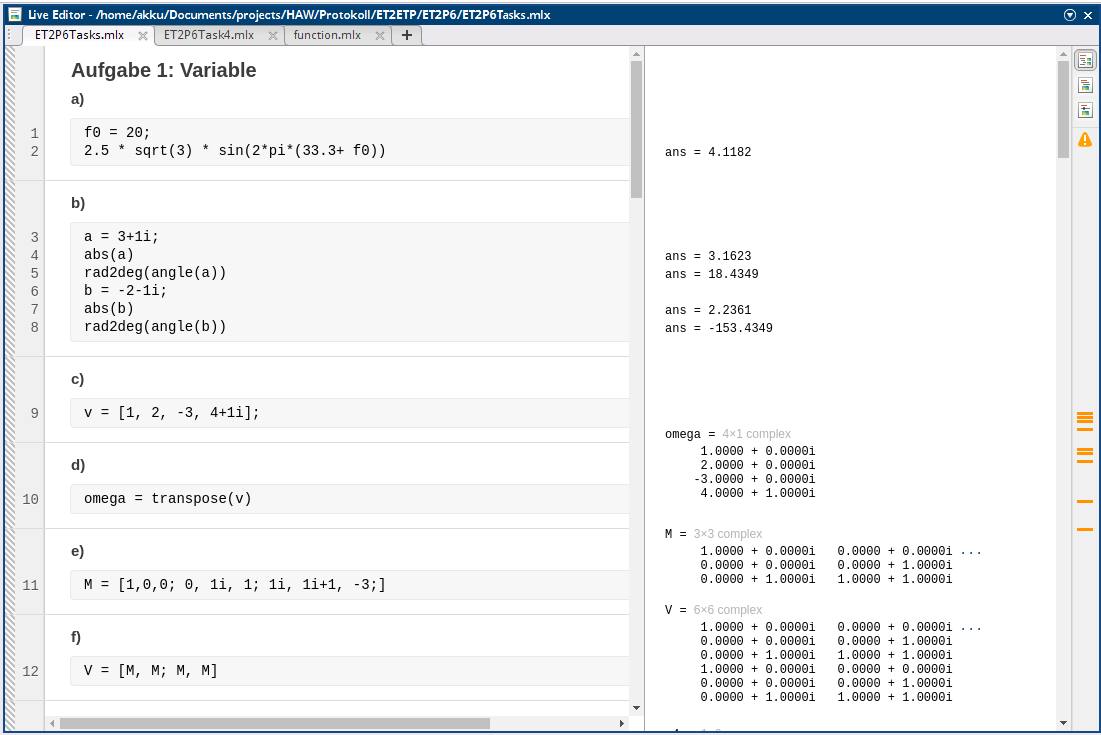
\includegraphics[width=\textwidth]{../assets/images/ET2P6/aufgaben1a_f.png}
  \caption{Die ersten Teile a)-f) von Aufgabe 1 mit den entsprechenden Ergebnissen daneben}
  \label{fig:auf1af}
\end{figure}
Wir erkennen leicht, dass die ersten Aufgaben von simpler Natur sind. Es werden vor allen Dingen kleinere, aber wichtige Funktionen und notwendige Kenntnisse über Notationen abgefragt.
\newpage
\begin{figure}[h]
  \centering
  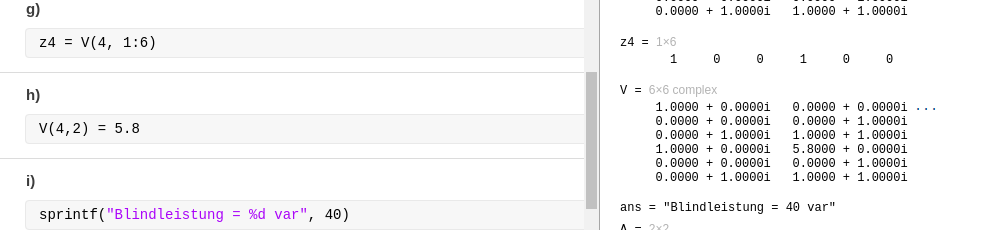
\includegraphics[width=\textwidth]{../assets/images/ET2P6/aufgaben1g_i.png}
  \caption{Die restlichen Aufgaben g)-i) von Aufgabe 1 mit den entsprechenden Ergebnissen daneben}
  \label{fig:auf1gi}
\end{figure}
Auch hier werden notwenige Grundlagen verlangt, die auch für das weitere Bearbeiten der Aufgaben von großer Wichtigkeit sind. Man bemerke hier, dass für Aufgabe h) die Änderung des Eintrags an der spezifischen Stelle in dem Auszug der Matrix zu sehen ist (siehe Abbildung \ref{fig:auf1gi}(vierte Zeile, zweite Spalte)).

\section{Aufgabe 2: Mathematische Operationen}

\begin{task}
  TIn der nächsten Aufgabe wollen wir uns mit den mathematischen Operationen beschäftigen, die uns in Matlab zur Verfügung stehen.
\end{task}

\begin{figure}[h]
  \centering
  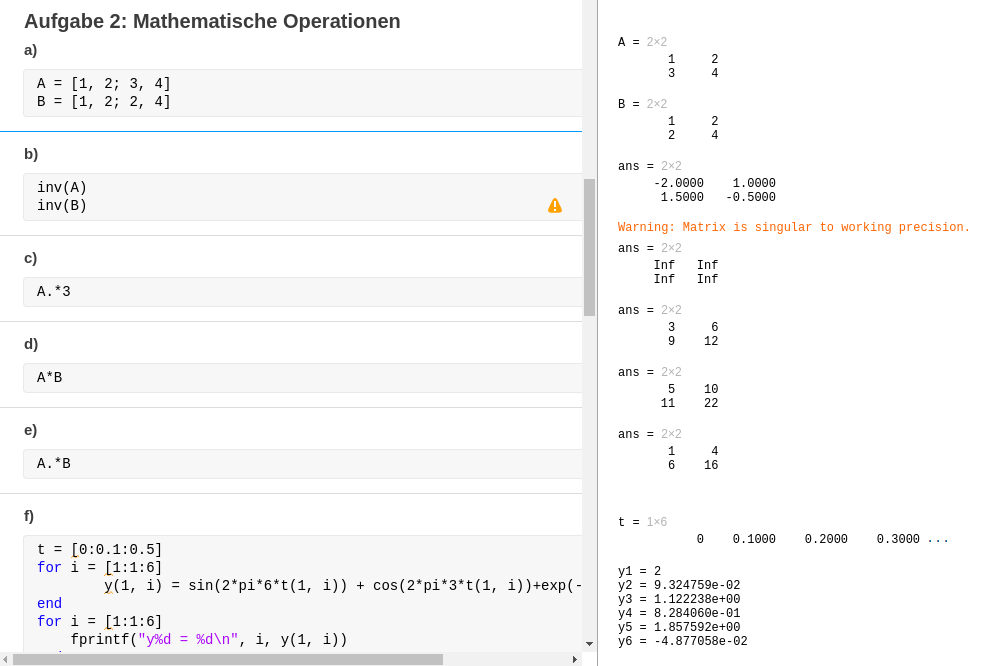
\includegraphics[width=\textwidth]{../assets/images/ET2P6/aufgaben2a_f.png}
  \caption{Die ersten Teile a)-f) von Aufgabe 2 mit den entsprechenden Ergebnissen daneben}
  \label{fig:auf2af}
\end{figure}

Neben dem Anlegen von Variablen und das Anwenden von intuitiven Funktionen

\end{document}
